\section{Location Transparency}
\subsection{Distributed Management/Retrieval of Data}
Challenges: 
\begin{itemize}
  \item Location: Where shall the item be stored?
  \item Location: How can the item be found?
  \item Scalability: keep the complexity for communication and storage scalable
  \item Robustness and resilience in case of faults and frequent changes
\end{itemize}

\subsection{Strategies for Data Retrieval}
Strategies to store and retrieve data items in distributed systems:
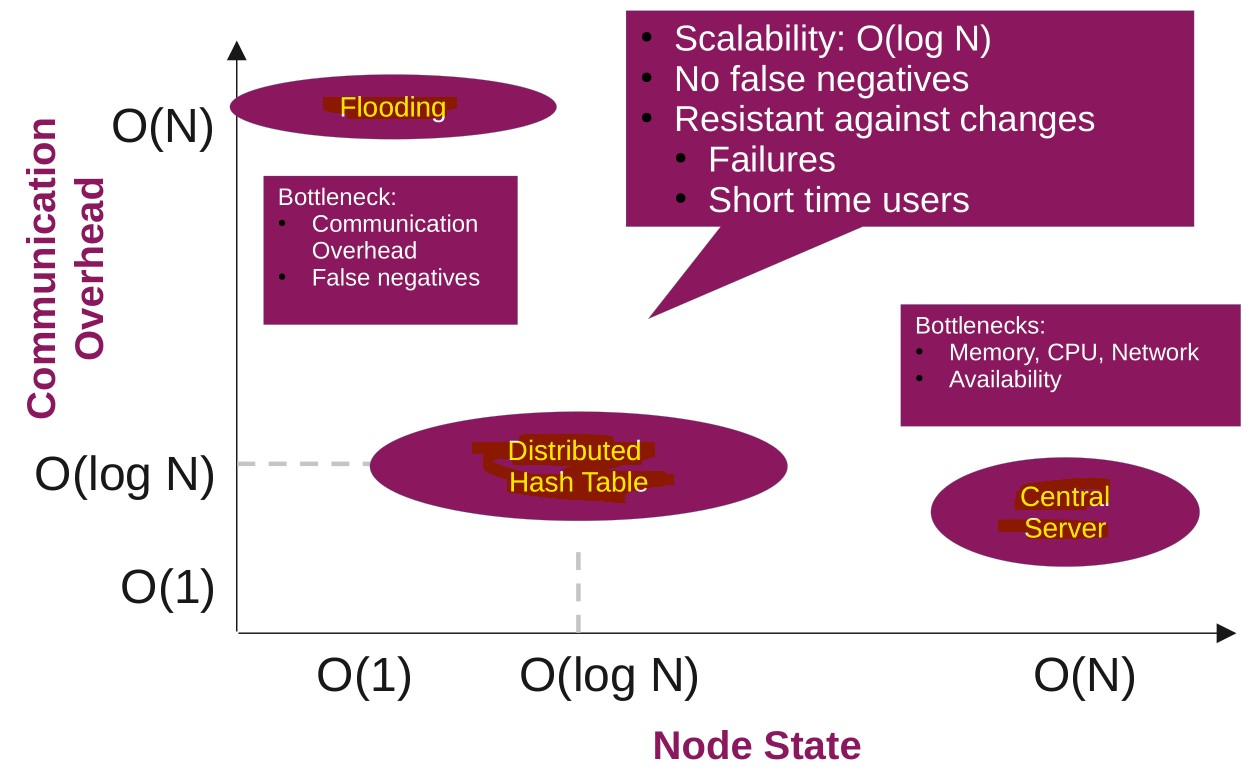
\includegraphics[width=\linewidth]{p2p-overview.jpg}
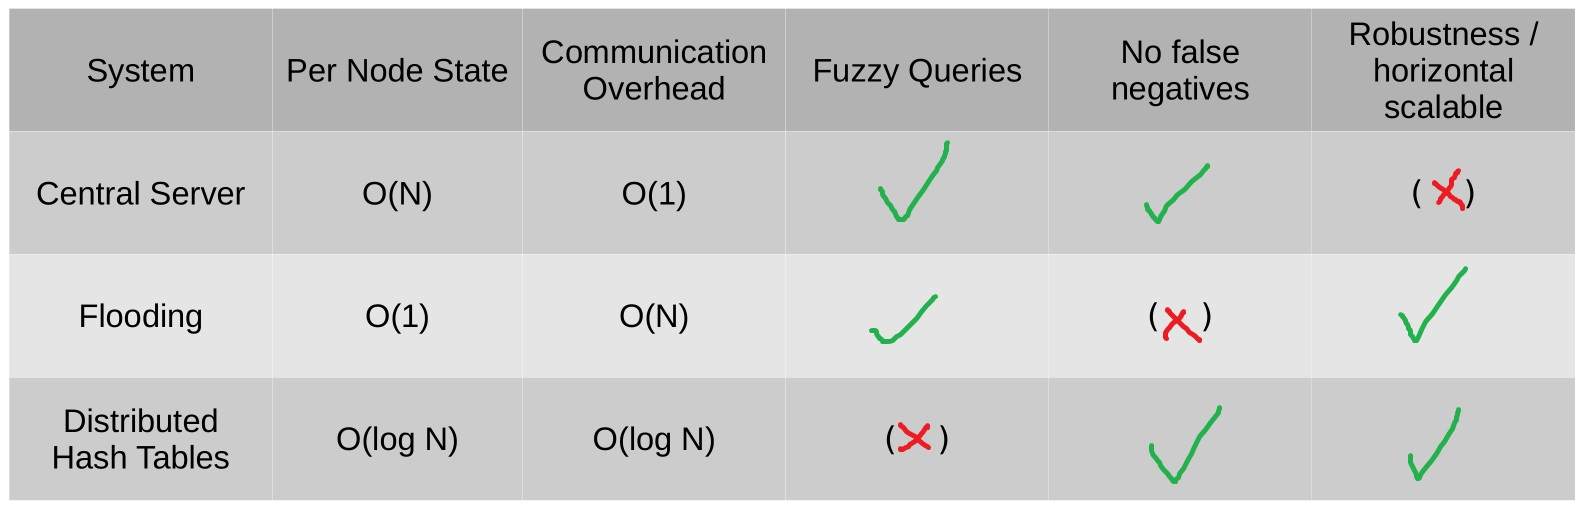
\includegraphics[width=\linewidth]{p2p-comparison.jpg}

\subsubsection{Central server}
e.g., service registry, reverse proxy - although main use case is load balancing.
Simple strategy: Central Server (can be powerful - vertical scaling!).
Server stores information about locations:
\begin{enumerate}
  \item Node A (provider) tells server that it stores item D
  \item Node B (requester) asks server S for the location of D
  \item Server S tells B that node A stores item D
  \item Node B requests item D from node A
\end{enumerate}
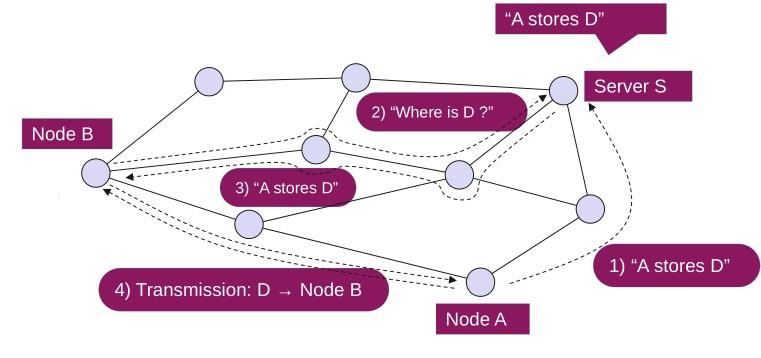
\includegraphics[width=\linewidth]{p2p-central-server.jpg}
\paragraph{Advantages}
\begin{itemize}
  \item Search complexity of O(1) - ``just ask the server''
  \item Complex and fuzzy queries are possible
  \item Simple and fast
\end{itemize}
\paragraph{Problems}
\begin{itemize}
  \item No Scalability
  \begin{itemize}
    \item O(N) node state in server
    \item O(N) network and system load of server
  \end{itemize}
  \item Single point of failure or attack
  \item (Single) central server not suitable for systems with massive numbers of users
\end{itemize}


\subsubsection{Flooding search}
e.g., layer 2 broadcasting, wireless mesh networks, Bitcoin
Fully-distributed Approach and ppposite approach of central server. No information on location of a content.\\
Retrieval of data:
\begin{itemize}
  \item No routing information for content
  \item Necessity to ask as much systems as possible / necessary
  \item No guarantee to reach all nodes
  \item Flooding: high traffic load on network, scalability issues
\end{itemize}

\paragraph{How it works}
There is an search fee to prevent spamming.
\begin{enumerate}
  \item Node B (requester) asks neighboring nodes for item D
  \item  Nodes forward request to further nodes (breadth-first search / flooding)
  \item Node A (provider of item D) sends D to requesting node B
\end{enumerate}
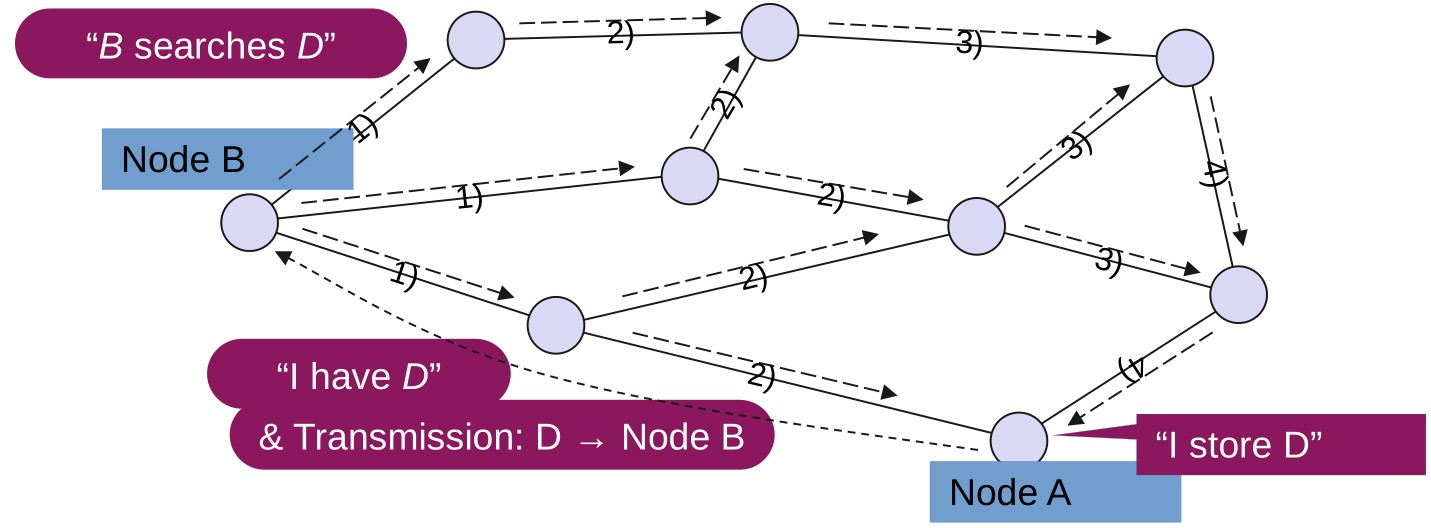
\includegraphics[width=\linewidth]{flooding.jpg}
\paragraph{For Bitcoin}
Bitcoin has all data in the block, so it searches itself.

\subsubsection{Distributed indexing / Hash Tables}
Tor, Bittorrent, IPFS, Apache Cassandra, Dynamo, Atek.\\

Goal is scalable complexity for:
\begin{itemize}
  \item Communication effort: O(log(N)) hops
  \item Node state: O(log(N)) routing entries
\end{itemize}

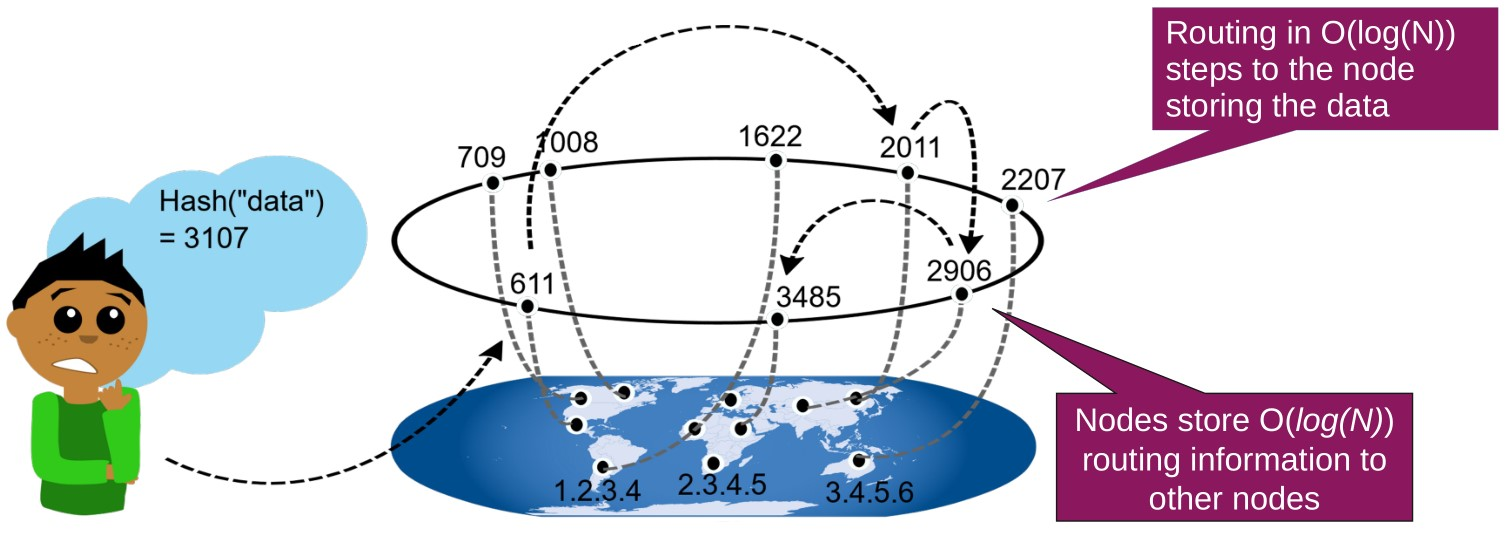
\includegraphics[width=\linewidth]{p2p-distributed-hash.jpg}
\begin{enumerate}
  \item Hash data
  \item Every node knows log(N) neighbors (for 1000, min. 3)
  \item First node asks neighbors
  \item Neighbors references next neighbor, and so on.
  \item Until node is found which is responsible for data item.
\end{enumerate}

\paragraph{Approach}
\begin{itemize}
  \item Data and nodes are mapped into same address space
  \item Nodes maintain routing information to other nodes
\end{itemize}
\paragraph{Problems}
\begin{itemize}
  \item Maintenance of routing information required
  \item Fuzzy queries not primarily supported
\end{itemize}
\paragraph{Characteristics}
\begin{itemize}
  \item Reliability / Scalability
  \item Equal distribution of content among nodes.
  \item Assignment of responsibilities to new nodes.
  \item Re-assignment and re-distribution of responsibilities in case of node failure or departure.
  \item Consistent hashing $\rightarrow$ nodes responsible for hash value intervals.
  \item More peers = smaller responsible intervals.
  \item Hash Table is something different.
\end{itemize}

\paragraph{Mapping of nodes and data}
\begin{itemize}
  \item Peers and content are addressed using flat identifiers: E.g., Address is public key (256bit) or SHA256 of public key. Content ID = SHA256(content)
  \item Nodes are responsible for data in certain parts of the address space
  \item Association of data to nodes may change since nodes may disappear
\end{itemize}
\subparagraph{Storing}
\begin{itemize}
  \item Each node is responsible for part of the value range:
  \begin{itemize}
    \item Often with redundancy (overlapping of parts)
    \item Continuous adaptation
    \item Real (underlay) and logical (overlay) topology are uncorrelated
  \end{itemize}
\end{itemize}
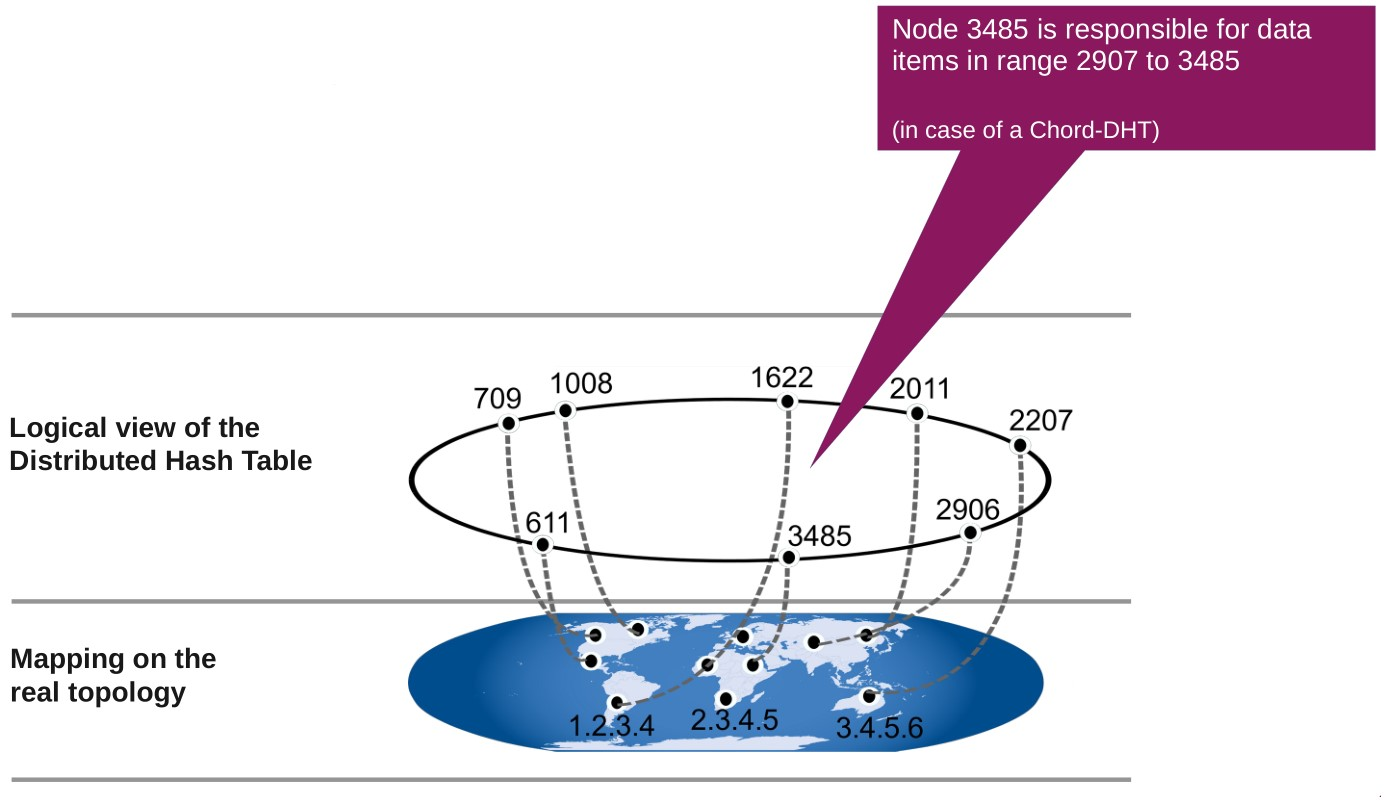
\includegraphics[width=\linewidth]{p2p-hash-table-topology.jpg}

\paragraph{Storing / Looking up data}
\begin{itemize}
  \item Store data = first, search for responsible node (Not necessarily known in advance)
  \item Search data = first, search for responsible node
\end{itemize}

\subparagraph{Routing to Data Item}
\begin{itemize}
  \item Start lookup at arbitrary node of DHT
  \item Routing to requested data item (key)
  \item K/V-pair is delivered to requester
  \item Requester analyzes K/V-tuple (and downloads data from actual location - in case of indirect storage)
\end{itemize}
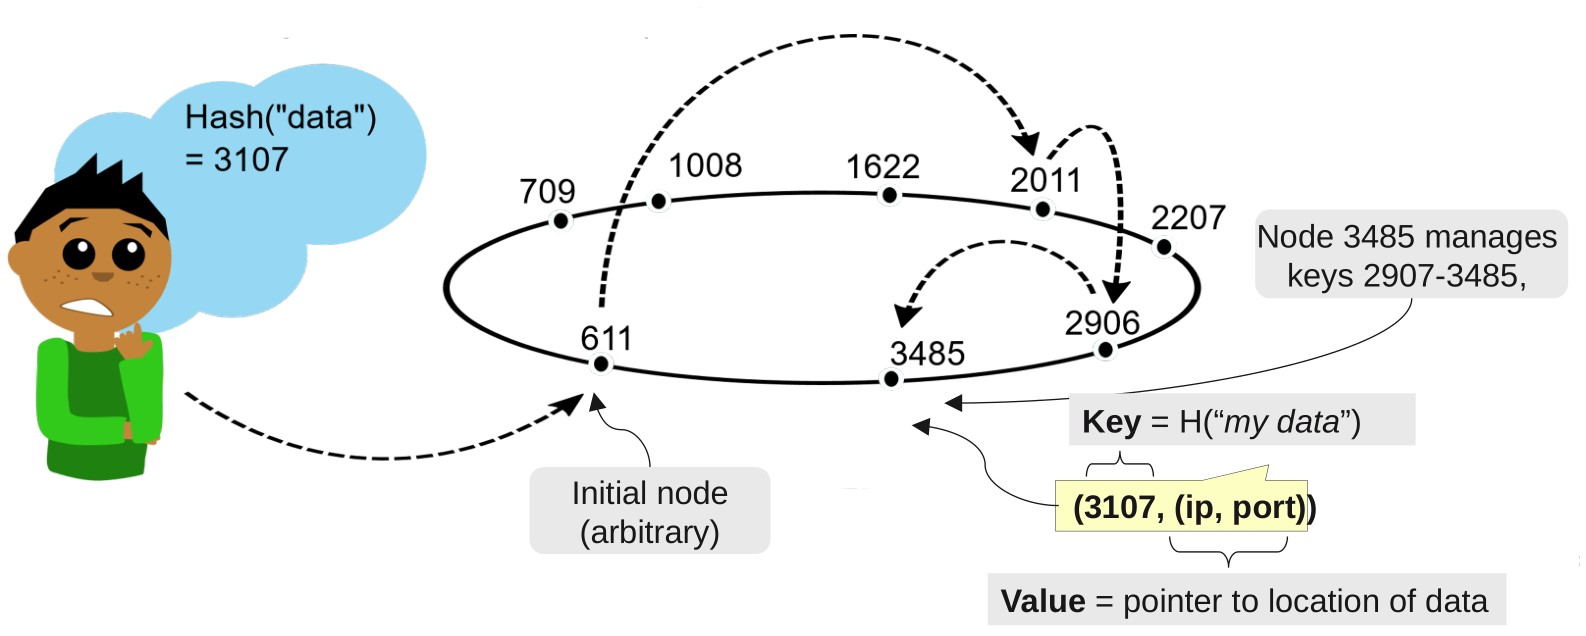
\includegraphics[width=\linewidth]{p2p-routing-to-data.jpg}

\textbf{Indirect vs Direct}:\\
Indirect is one step more: e.g.: Download from IP, Port. Good for larger files.\\
Direct is good for smaller files.

\paragraph{Join}
\begin{enumerate}
  \item Calculation of node ID (normally random / or based on PK)
  \item New node contacts DHT via arbitrary node (bootstrap node)
  \item Lookup of its node ID (routing)
  \item Copying of K/V-pairs of hash range (in case of replication)
  \item Notify neighbors
\end{enumerate}

\paragraph{Leave}
\subparagraph{Failure}
\begin{itemize}
  \item Use of redundant K/V pairs (if a node fails)
  \item Use of redundant / alternative routing paths
  \item Key-value usually still retrievable if at least one copy remains
  \item need for keep-alive messages
\end{itemize}
\subparagraph{Departure}
\begin{itemize}
  \item Copying of K/V pairs to corresponding nodes
  \item Friendly unbinding from routing environment
\end{itemize}

\paragraph{Kademlia}
Each Kademlia node and data item has unique identifier.
Keys are located on the node whose node ID is closest to the key.
Knows neighbors well, further nodes not that much.

\subparagraph{Example Search}
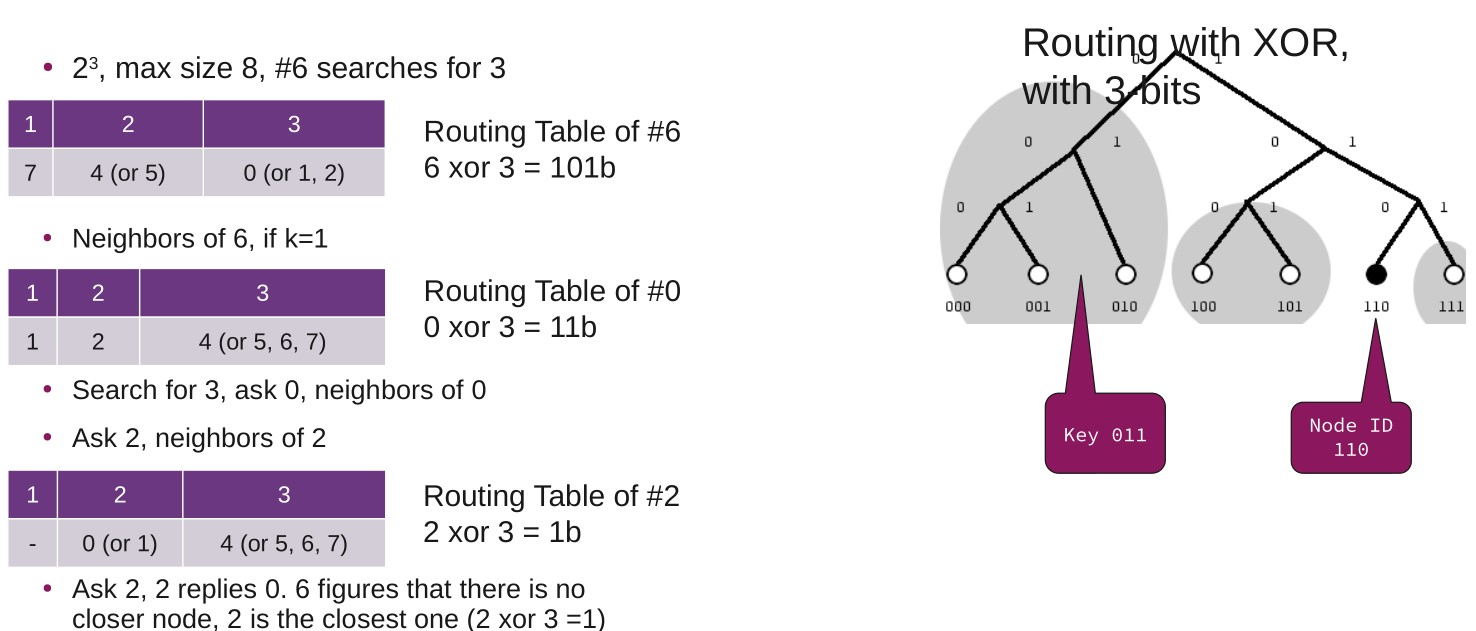
\includegraphics[width=\linewidth]{p2p-kademlia-example.jpg}

\paragraph{Sybil Attacks}
\begin{itemize}
  \item Create large number of identities
  \item Larger than honest nodes
  \item Isolate nodes
\end{itemize}
\subparagraph{Prevention}
\begin{itemize}
  \item Creation of identities costs money
  \item Always assume data from other nodes may be missing
  \item Chain of trust / reputation
\end{itemize}

\paragraph{Redundancy}
\subparagraph{Direct Replication}
\begin{itemize}
  \item Originator peer is responsible
  \item Periodically refresh replicas
  \item Example: tracker that announces its data
  \item Problem: Originator offline $\rightarrow$ replicas disappear. Content has TTL
\end{itemize}
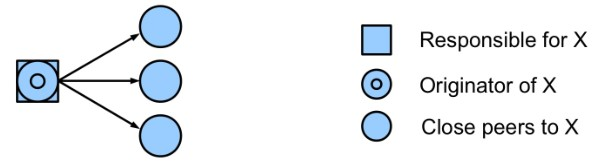
\includegraphics[width=\linewidth]{p2p-direct-replica.jpg}

\subparagraph{Indirect Replication}
\begin{itemize}
  \item The closest peer is responsible, originator may go offline vs any close peers are responsible.
  \item Periodically checks if enough replicas exist.
  \item Detects if responsibility changes.
  \item Problem: Requires cooperation between responsible peer and originator
  \item Problem: Multiple peers may think they are responsible for different versions $\rightarrow$ eventually solved
\end{itemize}

\subparagraph{Consistency in Replicas}
DHTs have weak consistency. 
If two changes are at the same time, one get overwritten.
Requires a coordinator. (Leader Election with tools)

\subsection{Similarity Search}
\subsubsection{Levenshtein Distance}
Example d(test,east) = 2 (remove a, insert t).\\
Main idea: pre-calculate errors:\\
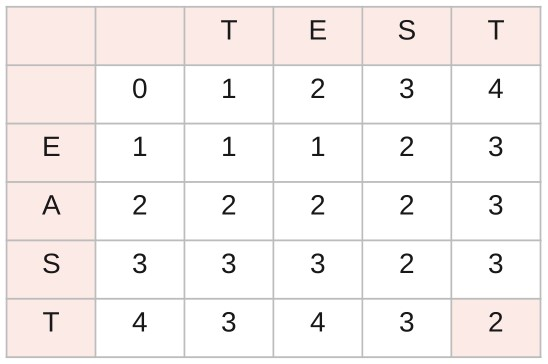
\includegraphics[width=\linewidth]{levenshtein-distance.jpg}
If Letters are the same: Calculate left or top and add one or select diagonal top-left and add 0. Select minimum. \\
If letters are not the same: select the minimum of either left, top, or diagonal top-left and add 1.

\subsubsection{FastSS}
FastSS pre-calculates with deletions only.
Neighbors for test with ed 2: test, est, st, et, es, tst, tt, ts, tet, te, tes.
11 neighbors → 11 more queries, indexed enlarged by 11 entries.\\
Example d(test,fest)=1\\
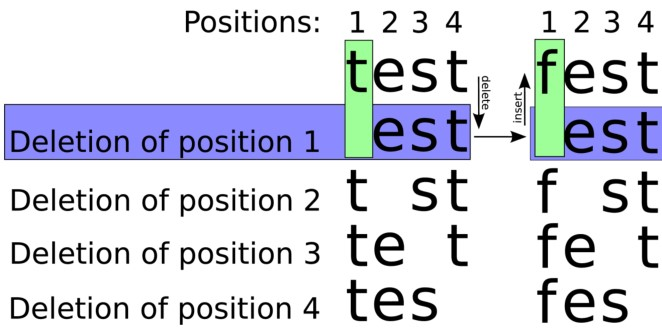
\includegraphics[width=\linewidth]{fastss-example-1.jpg}
Example d(test,east)=2\\
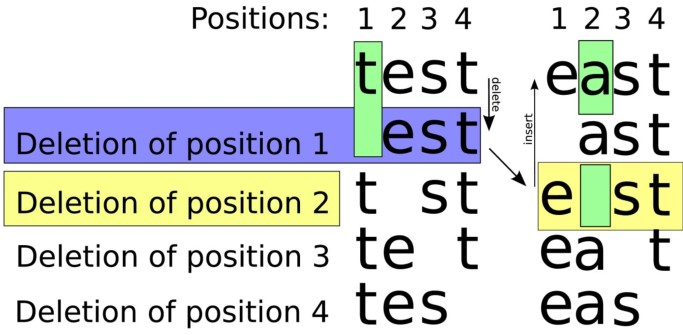
\includegraphics[width=\linewidth]{fastss-example-2.jpg}

\subsubsection{Range Queries}
Problem: random insert vs. sequence insert

\paragraph{Solution: Over-DHT}
DST: stores data on each level (redundancy) up to a threshold

\subparagraph{Example DST}
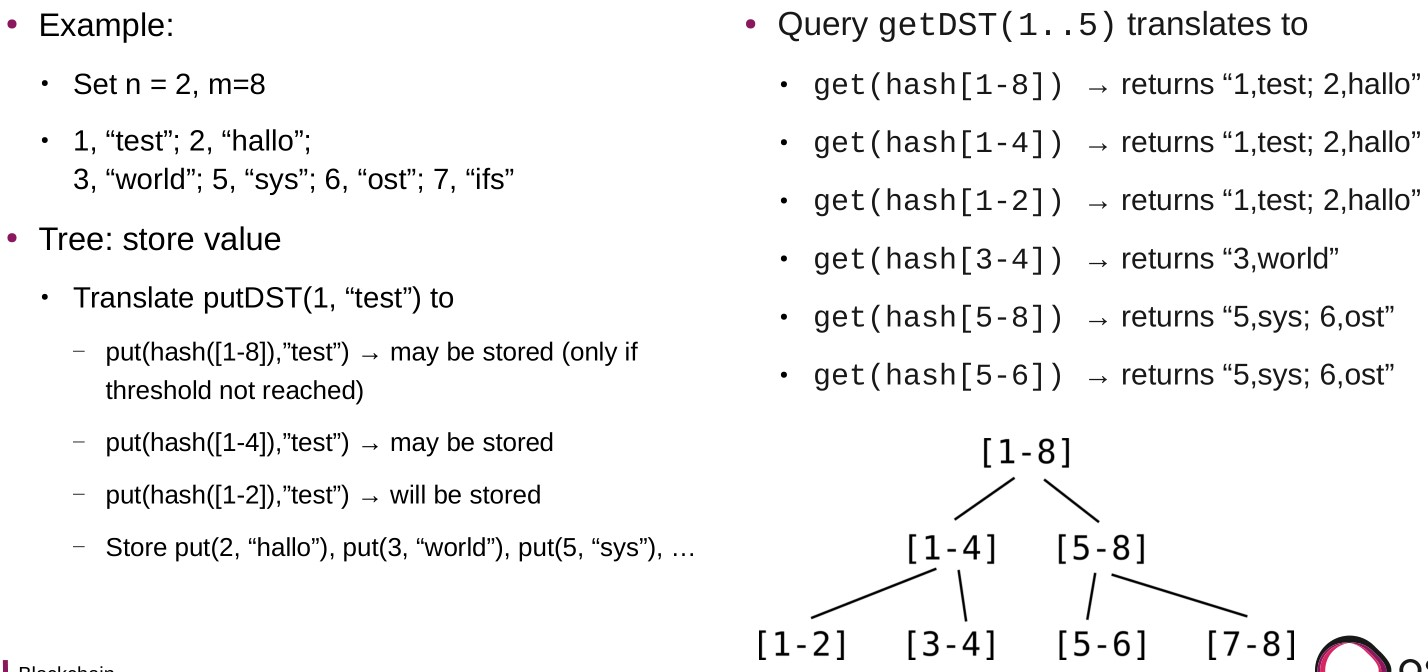
\includegraphics[width=\linewidth]{dst-example.jpg}